\documentclass{standalone}
\usepackage{hsbcommon}
\usetikzlibrary{calc}
\begin{document}
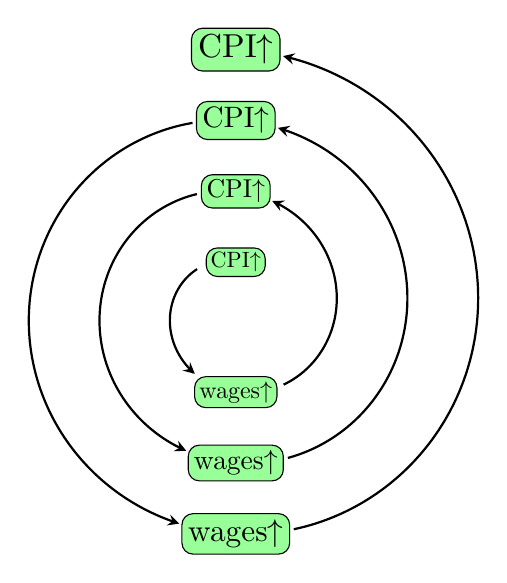
\begin{tikzpicture}[>=stealth]
    % spiral: angle = t+90, radius = 0.6 + t/400
    \foreach \t/\lab [count=\i from 0] in {0/CPI, 180/wages, 360/CPI, 540/wages,
                                           720/CPI, 900/wages, 1080/CPI} {
        \node[draw, rounded corners, fill=green!40,inner sep=2pt, scale={0.8+\t/2700}]
            (n\i) at ({\t+90}:{0.6+\t/400}) {\lab$\uparrow$};
    }
    % arrows from the side of one node to the side of the next
    \foreach \i [evaluate=\i as \j using int(\i+1),
                 evaluate=\i as \s using 180*\i] in {0,...,5} {
        \draw[->, thick]
            let \p1 = ($(n\i.east)-(n\i.west)$),
                \p2 = ($(n\j.east)-(n\j.west)$),
                \n1 = {scalar(\s + asin((0.5*\x1+1pt)/((0.6+\s/400)*1cm)))},
                \n2 = {scalar(\s+180 - asin((0.5*\x2+1pt)/((0.6+(\s+180)/400)*1cm)))}
            in plot[domain=\n1:\n2, samples=60, smooth, variable=\t]
                ({\t+90}:{0.6+\t/400});
    }
\end{tikzpicture}
\end{document}